%%%%%%%%%%%%%%%%%%%%%%%%%%%%%%%%%%%%%%%%%%%%%%%%%%%%%%%%%%%%%%%%%%%%%%%%%%%%%%%%%%%%%

\section{Evolution of Multimodal Learning}
Multimodal learning is a type of \textit{deep learning} that processes multiple types of data referred as modalities \cite{multimodal_learning_wiki}. That data may belong to different domain such as text, audio, images or video. Multimodal learning was proposed at the beginning of the DL period, around year 2011, whilst have raised their popularity when they were mixed with large multimodal languages in the recent years. 

\subsection{Multimodal deep Boltzmann machines}
Boltzmann machines are known to be the multimodal data dealing algorithm ancestors. Invented in 1985 and named after the \textit{Boltzmann distribution}, these machines can be seen as stochastic neural networks. Multimodal deep Boltzmann machines can process and learn from different types of information simultaneously, having a separate machine for each modality. Its units are divided into visible and hidden units, units which represent neurons with a binary output indicating whether they are activated or not.

\begin{figure}[H]
	\centering
	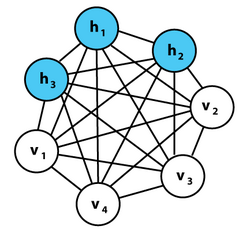
\includegraphics[width=0.3\textwidth]{imgs/boltzmann.png}
	\caption{Deep Boltzmann machine.}
	\label{fig:boltzmann_machine}
\end{figure}

However, learning is impractical using these machines because of the exponential computational time and not optimized architecture. Successor \textit{restricted Boltzmann machine} alternative was designed to deal with efficiency by just allowing connections between hidden units and visible units. Lowering the computational power and making training more efficient.

\subsection{Multimodal Transformers}
Transformers can also be adapter for modalities, usually finding a way to \textit{tokenize} the data domain. Even if multimodal transformers can be trained from scratch, a 2022 \textit{transfer learning} study showed that fine-tuned transformers originally pretrained with natural language data can show competitiveness in logical and visual tasks. 

\subsubsection{The Perceiver}
\label{sec:perceiver}
Perceivers, are a variant of the transformer architecture exclusively adapted for processing multimodal data. The Perceiver is designed as a general architecture that can learn simultaneously from large amounts of heterogeneous data, implementing \textit{asymmetric attention} mechanisms. Asymmetric attention consists of architectural modifications that break the "standard symmetry" to address specific domain constraints. This approach leads to outperforming specialized models on classification tasks. It iteratively alternates cross-attention and latent self-attention blocks to project a high-dimensional input byte array to a fixed-dimensional latent bottleneck before processing it using a deep stack of transformer-style self-attention blocks in the latent space \cite{jaegle2021perceivergeneralperceptioniterative}. 

\begin{figure}[H]
	\centering
	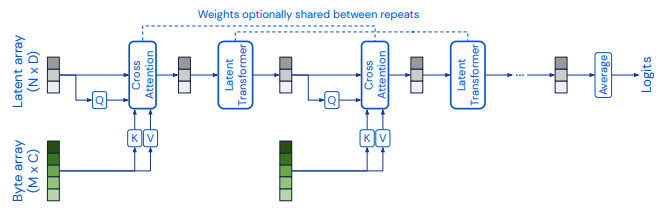
\includegraphics[width=0.9\textwidth]{imgs/Perceiver.png}
	\caption{Perceiver architecture from the referenced paper}
	\label{fig:perceiver_architecture}
\end{figure}

\subsubsection{Image generation Transformer models}
\begin{itemize}
	\item \textbf{DALL-E 1} (2021): When it comes to image generation models, \textit{DALL-E 1} is not a \textit{difussion model} (latent variable generative models). It uses a decoder-only transformer which autoregressively generates a text followed by the token representation of an image, which is ten converted by a variational autoencoder to an image. 
	
	\item \textbf{Parti} (2022): On the other hand, models like \textit{Parti} use an encoder-decoder schema. Where the encoder processes a text prompt and the decoder generates the token representation of an image.
	
	\item \textbf{Muse} (2023): uses an encoder-only architecture trained to predict the masked image tokens from unmasked image tokens. In training, all input tokens are masked, and the highest confidence predictions are revealed 
		
	\item \textbf{Phenaki} (2023): is a text-to-video-model which uses a bidirectional masked transformer conditioned on pre-computed text tokens. Then, the tokens are decoded to a video. 
\end{itemize} 

\subsection{Applications of Multimodal Learning}
The integration of data from different domains has allowed a deeper understanding of models for different type of tasks requiring multimodality:

\begin{itemize}
	\item \textbf{Cross-modal retrieval}: is a subfield of information retrieval which enables users to search and retrieve information across different data modalities \cite{cross_modal_retrieval}. Differing from the traditional retrieval systems, cross-modal retrieval bridges different types of media to facilitate flexible information access. There are several combinations of retrieval depending on both the input and output data domain, e.g. \textit{audio-to-video, video-to-text, ...}
	
	\item \textbf{Content generation}: models such as \textit{DALL-E} generate images from textual descriptions. 
	
	\item \textbf{Classification and missing data retrieval}: multimodal \textit{Deep Boltzmann Machines} outperform traditional shallow machine learning algorithms like the \textit{support vector machines} in classification tasks and are able to predict missing instances in multimodal datasets. 
	
	\item \textbf{Robotics and human-computer interaction}: multimodal learning has improved the interaction in robotics and AI by integrating sensory inputs like speech, vision and touch, aiding autonomous systems and human-computer interaction.
\end{itemize}

%%%%%%%%%%%%%%%%%%%%%%%%%%%%%%%%%%%%%%%%%%%%%%%%%%%%%%%%%%%%%%%%%%%%%%%%%%%%%%%%%%%%%
 
\section{Advancements of Vision Language Models}
While the multimodal models mentioned before established the standard workflow for processing heterogeneous data, they often treated modalities independently to be combined or translated. The next step in the evolution are the \textit{Vision Language Models}, representing a shift towards a more reasoning approach rather than bare multimodal output goals. Instead of just generating an image from text or retrieving text from a video, VLMs think across all the domains simultaneously, implementing the reasoning capabilities from \textit{large language models} to interpret visual scenes. 

VLMs are the result of the evolution to earlier image captioning systems, systems which were designed primarily to take isolated images and produce descriptions. However, this systems just received the image as input, not an image-text pair input as the vision language models do now \cite{wiki:Vision-language_model}. I will now go over some of the huge advancements that resulted when transitioning from the traditional multimodal learning to these new vision language models and their main differences:

\begin{itemize}
	\item \textbf{Different input handling}: while with multimodal learning you would have a separate model for handling data from a specific domain e.g. one for dealing with text and another for video, VLMs were designed to receive input pairs of data from different modalities. Usually being (image, text) pairs. The VLM is able to align concepts belonging to different modalities inside a single shared vector space. 
	
	\item \textbf{Change of objective}: multimodal learning mainly covered traduction problems from one domain to another, whereas modern VLMs seek inter-domain reasoning. The capability to reason and distinguish the same concept in different modalities.
	
	\item \textbf{Representation in the latent space}: vision language models try to preserve the same mathematic meaning for the same concept across all domains. 
\end{itemize}

\subsection{Earliest models}
The early image captioning systems from around year 2010 used the \textit{encoder-decoder} architecture, which will be described later on. These models would encode the patched images and vectorize them into feature vectors, which were then fed to the decoder part in order to generate the associated output description. When it comes to the strategies implemented by this earliest models include combination of handcrafted \textit{visual features} to encode the image patches and \textit{n-gram} templates to generate the description. 

Those visual features can refer to any visual property like points, edges or even objects in the image. % explain a little bit more?

On the other hand, n-grams are statistical language models that calculate the probability of the next word in a sequence from a fixed size window of previous words. Depending on the number of previous words considered, we can get bigram models if just one previous word is considered, if it's two is a trigram model, ... up to \textit{n} - 1 considered as \textit{n-gram} models and finally an unigram if no previous context is considered. 

The general approximation for a sequence of words $w_1, \dots, w_m$ is:
\[
P(w_1, \dots, w_m) \approx \prod_{i=1}^{m} P(w_i \mid w_{i-(n-1)}, \dots, w_{i-1})
\]

\begin{itemize}
	\item Unigram Model ($n=1$): No context, independent probabilities.
	\[
	P(w_1, \dots, w_m) \approx \prod_{i=1}^{m} P(w_i)
	\]
	
	\item Bigram Model ($n=2$): Depends on the single previous word.
	\[
	P(w_1, \dots, w_m) \approx \prod_{i=1}^{m} P(w_i \mid w_{i-1})
	\]
	
	\item Trigram Model ($n=3$): Depends on the two previous words.
	\[
	P(w_1, \dots, w_m) \approx \prod_{i=1}^{m} P(w_i \mid w_{i-2}, w_{i-1})
	\]
\end{itemize}

\subsection{Deep learning based models}
When the deep learning neural networks arose and became dominant near year 2015, newer models and strategies also emerged. Convolutional neural networks (CNNs) started to being used for image encoding and recurrent neural networks (RNNs) to generate the captions. 

Despite their respective success in independent tasks, the combination of both models hit a plateau when dealing with VLM scenarios due to their infrastructure limitations. Convolutional neural networks work great when capturing local spatial patterns but they struggle with global long-term dependencies of the whole image without a large number of layers. On the other hand these \textit{seq2seq} models performed poorly with long-term dependencies due to their hard-coded sequentiality. Often leading to the model forgetting the processes carried in the first layers of the architecture. 

% Explain CNNs and RNNs?

\subsection{The Transformers architecture Standard}
The transition from sequential models combined with convolutional neural networks to \textit{Transformers} solved the long-term dependency capturing issues and lack of global visual feature captioning. Still using these models, VLMs are able to attend to the whole input prompt simultaneously thanks to parallelization and attention mechanisms and also due to the specific vision transformer architectures. 

% necessary to explain the transformers architecture?
% Before going in detail of the components, I will go over the basic architecture most of the VLMs are based on: \textit{transformers}. Its functionality can be summarized in three stages:

The functionality of the basic Transformers architecture can be wrapped into three main stages: 

\begin{enumerate}
	\item The encoders transform the input sequence into high-dimensional numerical representations called \textit{embeddings} which capture all the semantic and positional meaning of the tokens belonging to the input. In order to deal with those high-dimensional embeddings in the next steps of the architecture where the order of the input sentence words cannot be distinguished as the transformer processes all tokens in parallel, the \textit{positional encoding} was implemented. These encodings typically use sine and cosine functions of different frequencies to provide a unique signature for each position:
	\[
	PE_{(pos, 2i)} = \sin(pos / 10000^{2i/d_{model}})
	\]
	\[
	PE_{(pos, 2i+1)} = \cos(pos / 10000^{2i/d_{model}})
	\]
	This ensures that the model captures the structural context (e.g., distinguishing between "dog bites man" and "man bites dog") before any attention is calculated.
	
	\item Then they use a mechanism called \textit{self-attention} which allows the encoder to focus on the most relevant tokens of the sequence independent of their position. This is where the magic of the transformers actually happens. The implementation of the attention mechanism replaced the use of previous \textit{seq2seq} models which relied on recurrence. The original paper also introduced the concept of \textit{scaled dot-product attention}: 
	
	$$\text{Attention}(Q, K, V) = \text{softmax}\left(\frac{QK^T}{\sqrt{d_k}}\right)V$$
	
	where respectively $Q, K, V$ are the query, key and value matrices, and $d_{k}$ the dimensionality value. This approach eliminates the need for RNNs, ensuring parallelizability for the architecture. In the self-attention mechanism, those matrices are dynamically generated for each input sequence, allowing the model to focus on the different parts of the input sequence at different timesteps. \textit{Multi-head attention} enhances the process by introducing several parallel attention heads simultaneously, enabling each head to learn different Q, K and V matrix linear projections and focusing on multiple aspects instead of a single one. MHA ensures that the input embeddings are updated from a more varied and diverse set of perspectives, and after the attention outputs are calculated, they are concatenated and passed through a linear layer transformation to generate the output. 
	
	\item Finally the decoders of the transformers take both the output of the self-attention mechanism and the encoder generated embeddings to generate the most statistically likely output sequence. In the case of VLMs, it can also use those attention-weighted embeddings to output the most loyal visual representation compression.
\end{enumerate}

\begin{figure}[H]
	\centering
	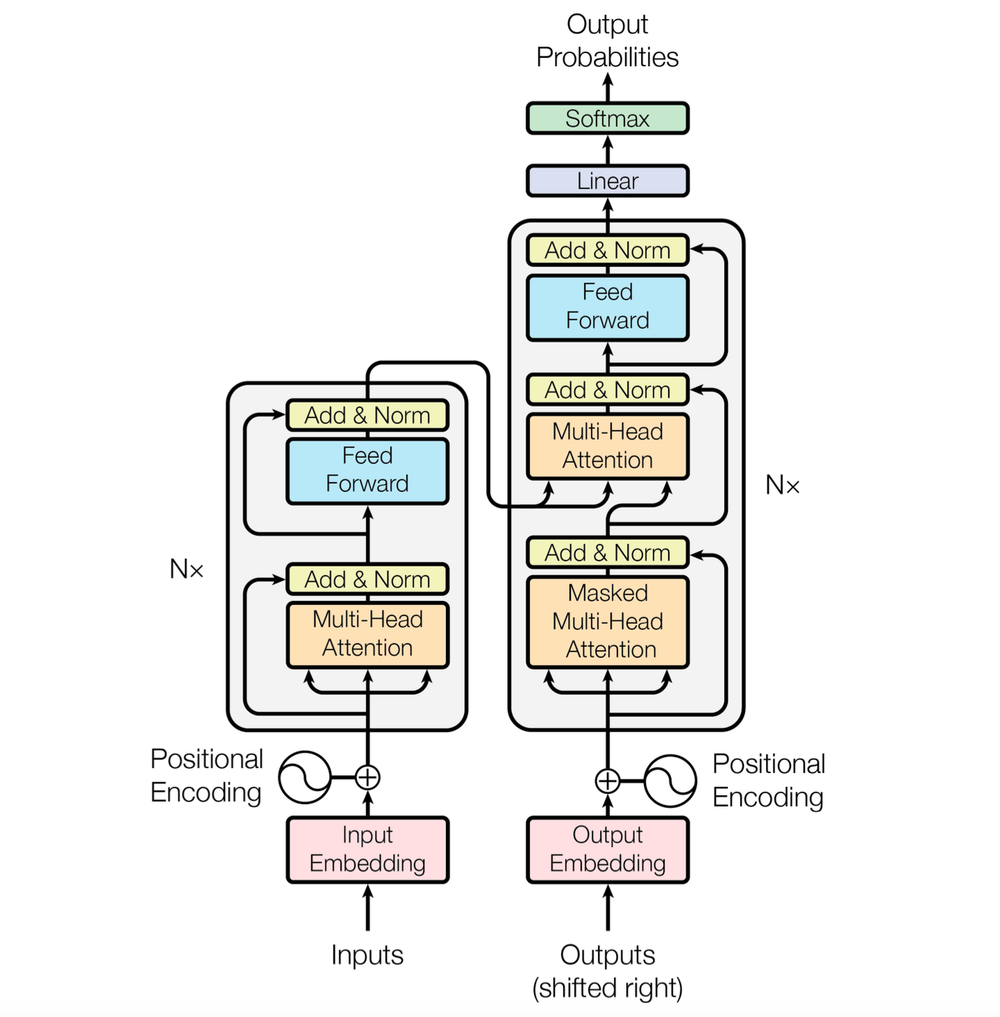
\includegraphics[width=0.6\textwidth]{imgs/The-Transformer-model-architecture.png}
	\caption{Original Transformers architecture published in \textit{"Attention is all you need"}}
	\label{fig:transformer_architecture}
\end{figure}

\subsubsection{VLM tasks with Transformers} 
The transformer architecture replaced the sequential recurrent neural networks in the role as decoders. In parallel, the network parameter training started relying on image-text pair datasets, and the scope of VLMs widened until reaching other tasks. 

\begin{itemize}
	\item \textbf{Phrase grounding}: Among those tasks, \textit{phrase grounding} could be mentioned. Task involving both natural language processing and computer vision where words or phrases within a sentence are associated to corresponding patches in an image \cite{timothy2024phrasegrounding}. Consists of identifying the spatial location within an image that aligns with the meaning of a given phrase, enabling models to map visual and textual data. 
	
	\begin{figure}[H]
		\centering
		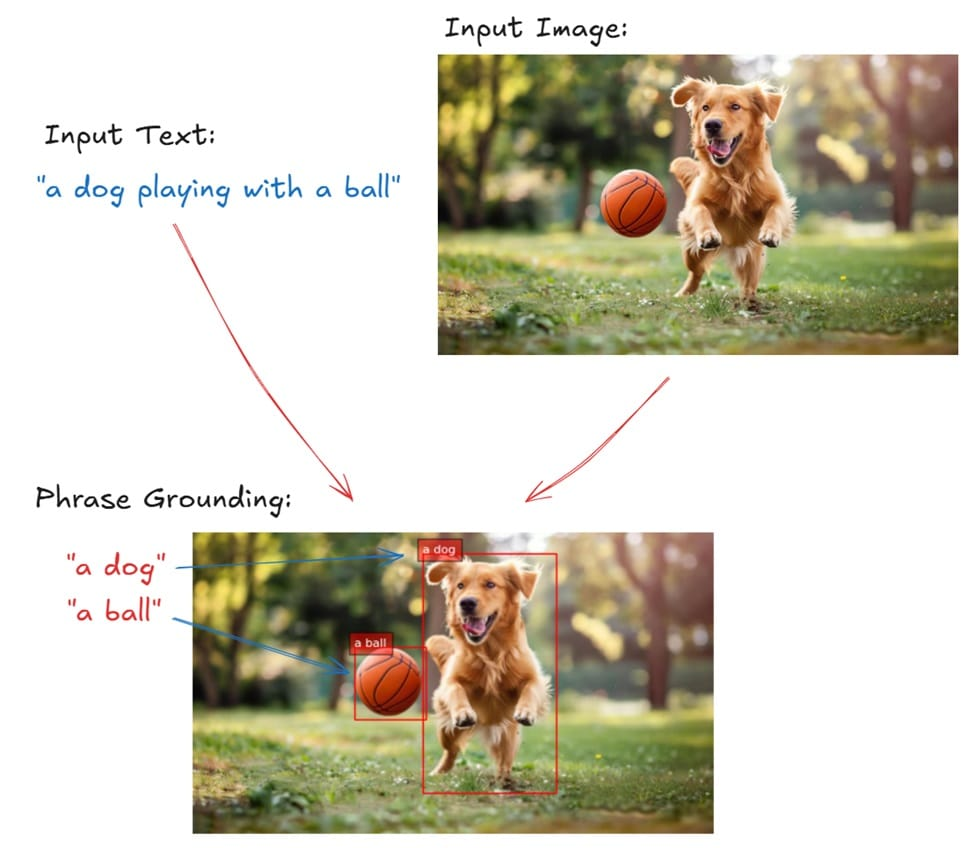
\includegraphics[width=0.5\textwidth]{imgs/phrase_grounding.jpg}
		\caption{Graphical example of phrase grounding.}
		\label{fig:phrase_grounding_example}
	\end{figure}
	
	\item \textbf{Visual Question Answering} (VQA): Another task which still remains as perhaps the most relevant one is \textit{visual question answering}. Specific task where the model is provided with an image and a specific related question, and it must generate an accurate response to it based on the visual content. Being its core pillars the object detection duty for identifying the objects in the image, then scene understanding to map the relations between objects and then finally text comprehension for embedded text interpretation within an image \cite{gravio2025vlmvqa}. 
	
\end{itemize}

However, modern VLMs do not follow the conventional 2017 paper \cite{vaswani2023attentionneed} workflow, they typically use different transformers configuration. Some models use only the encoder part of the architecture for both modalities, completely ignoring the traditional encoder component. While other recent models use the encoder for feature extraction and use an independent encoder for language modeling. Different approaches that will be explained in the following sections. 

%%%%%%%%%%%%%%%%%%%%%%%%%%%%%%%%%%%%%%%%%%%%%%%%%%%%%%%%%%%%%%%%%%%%%%%%%%%%%%%%%%%%%

\section{From Encoders to Generative LLMs}
\subsection{Language encoder} 
In traditional multimodal systems, the language encoder functioned as a bidirectional processor, having the role of generating contextualized latent representation of the input where each token could attend to its surrounding tokens in both directions. However, in modern VLM architectures, the encoder has been linked to the LLM engine. Functioning as a preparation of the linguistic information to interact with the visual tokens within a shared vectorial space.  

\subsection{The LLM transition: from encoders to decoder-only architectures}

The most significant paradigm shift in VLM evolution is the transition from symmetric \textit{encoder-decoder} systems to \textit{decoder-only} architectures. This move toward generative LLMs is driven by three fundamental technical advantages:

\begin{itemize}
	\item \textbf{Causal Attention vs. Bidirectional Attention}: Unlike encoders that allow tokens to see the entire sequence at once, decoders implement a \textit{causal mask}. This ensures that during training and inference, each token can only attend to itself and preceding tokens. This directional dependency is what enables autoregressive generation, the ability to reason and predict the next word in a conversation.The causal mask $M$ is typically a lower triangular matrix, where the attention score between position $i$ and $j$ is set to $-\infty$ if $j > i$:
	\[ M_{ij} = \begin{cases} 0 & \text{if } i \geq j \\ -\infty & \text{if } i < j \end{cases} \]
	After applying the \textit{softmax} activation function, these $-\infty$ values become zero probability, effectively blocking information flow from future tokens.
	
	\item \textbf{In-Context Learning and Reasoning}: By utilizing a decoder-only system, the VLM treats the input image as a visual prefix. The model does not just classify the image, rather it predicts the logical continuation of a sequence $[Image, Instruction, Response]$. This allows the model to influence \textit{Chain-of-Thought} (CoT) reasoning, where it can articulate its thought process before arriving at a final answer.
	
	\item \textbf{Scalability and Unified Training}: Decoder-only models are simpler to scale because they consolidate the entire reasoning process into a single set of weights. In a model like \textit{LLaVA}, the LLM receives a unified sequence of tokens: $\mathcal{S} = [v_1, \dots, v_n, t_1, \dots, t_m]$, where $v$ represents aligned visual pseudo-tokens and $t$ represents text tokens. The model treats these two modalities as a single language, significantly reducing the architectural bottleneck between "seeing" and "speaking."
\end{itemize}

%%%%%%%%%%%%%%%%%%%%%%%%%%%%%%%%%%%%%%%%%%%%%%%%%%%%%%%%%%%%%%%%%%%%%%%%%%%%%%%%%%%%%

\section{Vision Transformers}
\subsection{Vision encoder \& Vision Transformers (ViT)} 
Compared to earlier VLMs which used \textit{convolutional neural networks} (CNNs) for feature extraction such as the colors, shapes and textures from the input, modern ones employ an architecture called \textit{visual transformer} (ViT). 

Visual transformers process images into smaller patches (rather than text tokens) and treats them as sequences, implementing also the self-attention mechanism across the patches to create a transformer-based representation of the input message.

ViTs were designed as \textit{convolutional neural network} alternatives in computer vision applications, having different biases, training stability and data efficiency. Compared to CNNs, vision transformers are less efficient yet they have higher capacity. 

The image available below \ref{fig:vit_architecture} references the original architecture published in the 2020 paper \cite{dosovitskiy2021imageworth16x16words}, being basically a \textit{BERT}-like encoder-only transformer. It also uses special token \texttt{<CLS>} in the input side to refer to the start of the sentence token, and the output vector is used as the input of the final MLP head. Transformers, including the ViTs, measure the relationship between pairs of input tokens with the attention mechanism. In the case of images, the basic unit of analysis is the pixel. Vision transformers compute relationships between small regions of pixels (patches) and they maintain the spatial order with the positional embeddings computation. Each section of the architecture is passed through a linear sequence and multiplied by the embedding matrix, being the result with the position embedding fed to the transformer. Let's overview its functionality:

\begin{enumerate}
	\item The input image is of type $\mathbb{R}^{H \times W \times C}$, where $H, W, C$ are height, width, and channel (RGB). It is then split into square-shaped patches of type $\mathbb{R}^{P \times P \times C}$. For each of the patches, the respective "patch embedding" is obtained by pushing the patch through a linear operator and transformed through the \textit{positional encoding} layer. Both embeddings are added and pushed to the various transformer encoder layers. 
	
	\item Inside those encoder layers, the attention mechanism incorporates more and more semantic relations to the image patch embeddings. 
	
	\item Depending on the end task desired, one could add different layers in the end steps. For instance, for a classification task like the one performed in the image, a shallow \textit{multi-layer perceptron} (MLP) layer is added on top to output the probability distribution over the classes. As fact, the original paper goes for a linear-GeLU linear softmax network for classification. 
	
\end{enumerate}

% geroko
\begin{figure}[H]
	\centering
	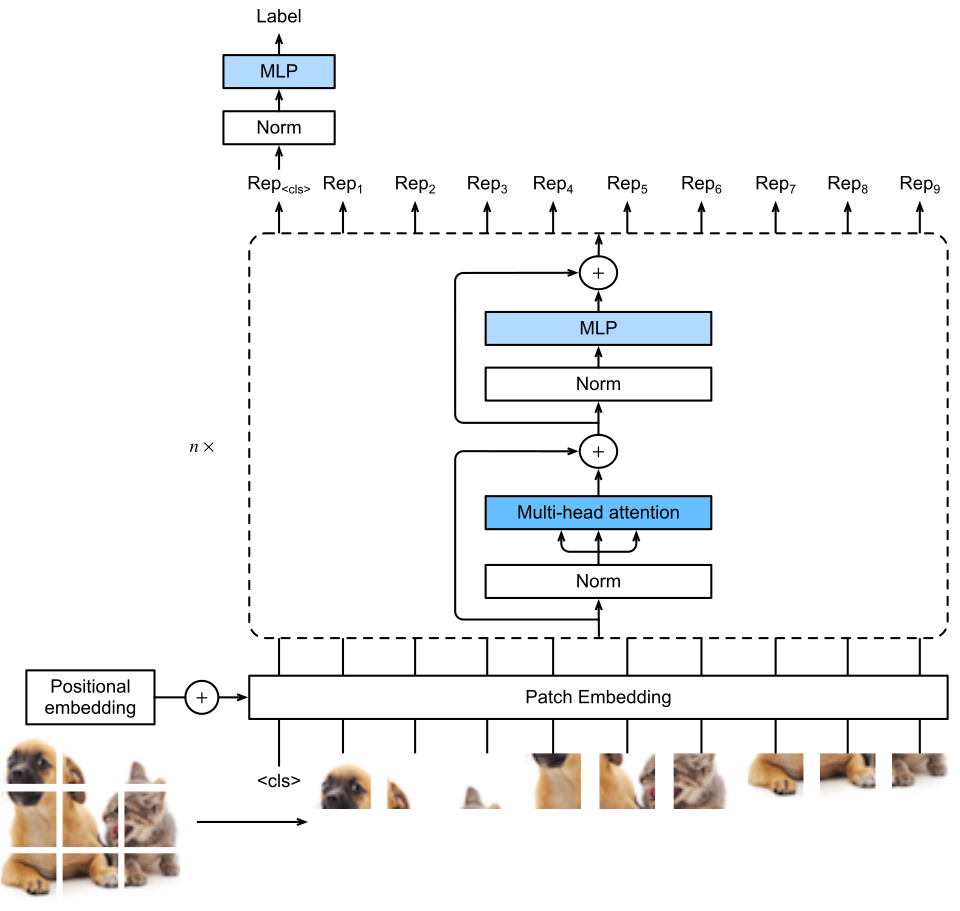
\includegraphics[width=0.7\textwidth]{imgs/Vision_Transformer.png}
	\caption{Vision transformer architecture}
	\label{fig:vit_architecture}
\end{figure}

There are other ViT variants which have been published and reported having used different techniques to deal with image manipulation. The following are some of the architectural improvements:

\begin{itemize}
	\item \textbf{Global average pooling (GAP)}: unlike the original paper where the \texttt{[CLS]} token is used to represent the beginning of the sequence emulating BERT, this approach does not use it. It simply takes the average of all output tokens as the final classification token. In the original report, it was mentioned to be equally efficient to the original approach. 
	
	\item \textbf{Multi-head attention pooling (MAP)}: it applies a new \textit{multi-head attention} block to pooling. It takes the output of the ViT this being the list of vectors $x_1, x_2, \dots, x_n$, whereas its output is $\text{MultiheadedAttention}(Q, V, V)$. Where \textit{Q} is the trainable query vector and \textit{V} the matrix with the rows being the input vectors. More recent papers state that both GAP and MAP show a better performance than the basic BERT-like pooling. 
	
	\item \textbf{Masked Autoencoder}: this architecture involves two vision transformers put end-to-end. The first one takes the input image patches with positional encoding and output the vectors representing each patch (same encoder procedure seen until now). This is where the second component being the decoder (even if it still an encoder-only transformer) takes the first encoder's output with positional encoding too and outputs the image patches again. See the architecture in the image below \ref{fig:masked_autoencoder_architecture}.
	
	\begin{figure}[H]
		\centering
		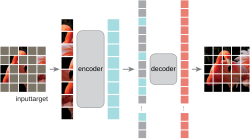
\includegraphics[width=0.6\textwidth]{imgs/Masked_Autoencoder..png}
		\caption{Masked autoencoder architecture}
		\label{fig:masked_autoencoder_architecture}
	\end{figure}
	
	During the training process, a percentage of the splitted patches is masked by special mask tokens, while leaving others untouched (the sweet spot has been said is around 75\% mask ratio). The whole network's task is to reconstruct the whole image with the missing "puzzle pieces" (being the masked patches). Masked patches are added back to the output of the encoder block as mask tokens and both are fed into the "decoder". A reconstruction loss is computed for the masked patches to assess network performance. In the prediction stage, the decoder is left over, the input image patches are processed and the resulting vector representation is fed to the encoder. 
	
	\item \textbf{DINO (self-DIstillation with NO labels)}: like the masked autoencoder procedure, DINO is a self-supervised way to train a vision transformer. Acting as a "teacher-student" method, the student being the model itself and the teacher, an exponential average of the student's past states, must be able to transfer its knowledge to the smaller model \cite{wiki:knowledge_distillation}. The loss function it uses is the \textit{cross-entropy loss} between the output of the teacher network and the output of the student version. The inputs of the networks are two different crops of the same image, represented as $T(x)$ and $T'(x)$, where $x$ is the original image. And as mentioned before, the network of the teacher represents the exponential decay average of the student's past parameters: 
	
	\begin{equation}
		\theta_{t'} = \alpha \theta_t + \alpha(1 - \alpha) \theta_{t-1} + \dots
	\end{equation}
	
	All put together, the loss function stands as followed:
	\begin{equation}
		\mathcal{L}(f_{\theta_{t'}}(T(x)), f_{\theta_{t}}(T'(x)))
	\end{equation}
	
	
\end{itemize}

In order to finish the ViT research subsection, I would like to make a little comparison with their "ancestor" model, the \textit{convolutional neural networks} (CNNs).

The fundamental distinction between Vision Transformers and the convolutional neural networks lies in their inductive biases. CNNs are built on the principles of locality and translation invariance, using sliding kernels that assume pixels close to each other are more related than those far apart. This bias allows CNNs to be highly efficient with smaller datasets and provides a natural robustness to local perturbations and noise. In contrast, ViTs discard these spatial assumptions. By treating an image as a sequence of patches and applying a global self-attention mechanism, a ViT can capture long-range dependencies between distant parts of an image from the very first layer. This flexibility allows ViTs to surpass CNN performance on massive datasets where the model can "learn" the spatial relationships from scratch, rather than having them hard-coded into the architecture.

However, this architectural freedom comes with a significant trade-off in terms of optimization and data requirements. Because ViTs lack the "shortcuts" provided by the convolutional structure, they are notoriously sensitive to hyperparameter choices and the selection of optimizers, often requiring advanced strategie and specific learning rate schedules to achieve stability. While a CNN's computational complexity scales linearly with the number of pixels, the self-attention in ViTs is quadratically complex $O(N^2)$ relative to the number of patches $N$, making high-resolution processing more resource-intensive. Consequently, while CNNs remain the more time-efficient and stable choice for many standard applications, ViTs have become the preferred backbone for large-scale Vision-Language Models due to their superior ability to scale and their capacity for modeling the complex, global context required for multimodal understanding.

%%%%%%%%%%%%%%%%%%%%%%%%%%%%%%%%%%%%%%%%%%%%%%%%%%%%%%%%%%%%%%%%%%%%%%%%%%%%%%%%%%%%%

\section{Multimodal Alignment: CLIP}
\subsection{CLIP: Contrastive Language-Image Pretraining}
In the year 2021, OpenAI launched the approach that would totally revolution the evolution of vision language models, they released the method of \textit{contrastive language-image pretraining} also known as \textit{CLIP}. Technique for training an image-text pair into neural network models, having an exclusive neural network for image and text understanding purposes, adopting a contrastive objective. 

When it comes to the algorithm itself, each neural network receives the input in the corresponding format and returns a single semantic/visual representative vector \cite{wiki:clip}. The objective to maximize by both models is the best alignment between both output vectors in the shared vector space, mapping the similar text-image pairs as close as possible while putting apart the most dissimilar ones. The training relies on a huge dataset with image-text pairs as and the two output vectors are considered similar depending on the \textit{dot product} value. 

% dot prodcut formula
\begin{equation}
	s_{i,j} = \mathbf{v}_i \cdot \mathbf{w}_j = \sum_{k=1}^{d} v_{i,k} w_{j,k}
\end{equation}
where $\mathbf{v}_i$ and $\mathbf{w}_j$ represent the embedding vectors generated by the text and image encoders respectively, and $d$ denotes the dimensionality of the vector space. The loss function used is the multi-class N-pair loss, which is a symmetric \textit{cross-entropy loss} over the similarity scores. The function fosters the dot product between the matching image and text vectors to be as high as possible, while discouraging high dot products between mismatching pairs. 

% loss function formula
\begin{equation}
	\mathcal{L} = -\frac{1}{N} \sum_{i} \ln \frac{e^{v_i \cdot w_i / \tau}}{\sum_{j} e^{v_i \cdot w_j / \tau}} - \frac{1}{N} \sum_{j} \ln \frac{e^{v_j \cdot w_j / \tau}}{\sum_{i} e^{v_i \cdot w_j / \tau}}
\end{equation}
being parameter \textit{T} the temperature parameter (\textit{T}>0) which is parametrized and learned during the training. Other loss functions are possible, such as the \textit{Sigmoid CLIP} function.

Once gone over the algorithm's properties, let's dive deep into the architecture:

\begin{itemize}
	\item \textbf{Image model}: when it comes to the image encoder used in most of the CLIP versions, they all usually are some kind of \textit{vision transformers} (ViT). Vision transformers often vary on the patch size, being that size the \textit{n}x\textit{n} dimensions of the patch the image was divided into. Alternatively, \textit{convolutional neural networks} (CNNs) can be used as well (such as \textit{ResNet}), the essential thing is to ensure the sizes of the image and text model output vectors are the same size. 
	
	\item  \textbf{Text model}: the text encoding models are usually \textit{transformers}. Even if it is heavily inspired by the transformers report published by OpenAI \cite{radford2021learningtransferablevisualmodels} and shares similarities with the \textit{GPT} architecture (decoder-only), the text model serves as a text encoder. Furthermore, its functionality is inspired by encoder only models such as \textit{BERT}, while sharing the dimensionality and number of parameters with decoder-only models as mentioned before. 
\end{itemize}

After going over the properties of both encoders that make the whole CLIP model, I will detail the model's workflow inspired on the image below \ref{fig:clip_architecture}. 

\begin{enumerate}
	\item The image of the image-text pair input is first splitted into smaller sized images named patches and then	fed into the vision encoder, which as mentioned earlier, can be any kind of architecture such as a vision transformer (ViT) or convolutional neural network (CNN). The output of the vision encoder will in fact be a vector representation of all the features that have been captured: shapes, texture, colors, objects, spatial relations, ... etc. 
	
	\item Now it's time the model turns those embeddings into real semantic representations, nevertheless, the model still does not know how to label concepts directly. So the model must know combine the embeddings obtained in the image model with the ones from the text model output, aligning them into a shared vector space establishing the real relations and links between the pairs. This bridging mechanism between the image and text pair (which will be described deeper in the corresponding section) is where the CLIP model's magic really shines. CLIP uses a contrastive alignment strategy in order to put correct pairs closer and dissimilar pairs further in the vector space.
	
	\item In the standard CLIP workflow, the model does not generate new text; instead, it performs \textit{zero-shot prediction} by calculating the similarity between the image embedding and a set of candidate text embeddings. It identifies which text snippet has the highest dot product with the image, effectively "selecting" the best label.
	
	\item In more advanced generative extensions, these aligned visual features are passed to an LLM. The LLM treats the image embeddings as part of its input sequence, allowing it to generate complex descriptions or provide answers to specific questions in a task known as \textit{Visual Question Answering} (VQA).
\end{enumerate}

% image of the CLIP architecture[H], dataset, preprocessing and other things later on.
\begin{figure}[H]
	\centering
	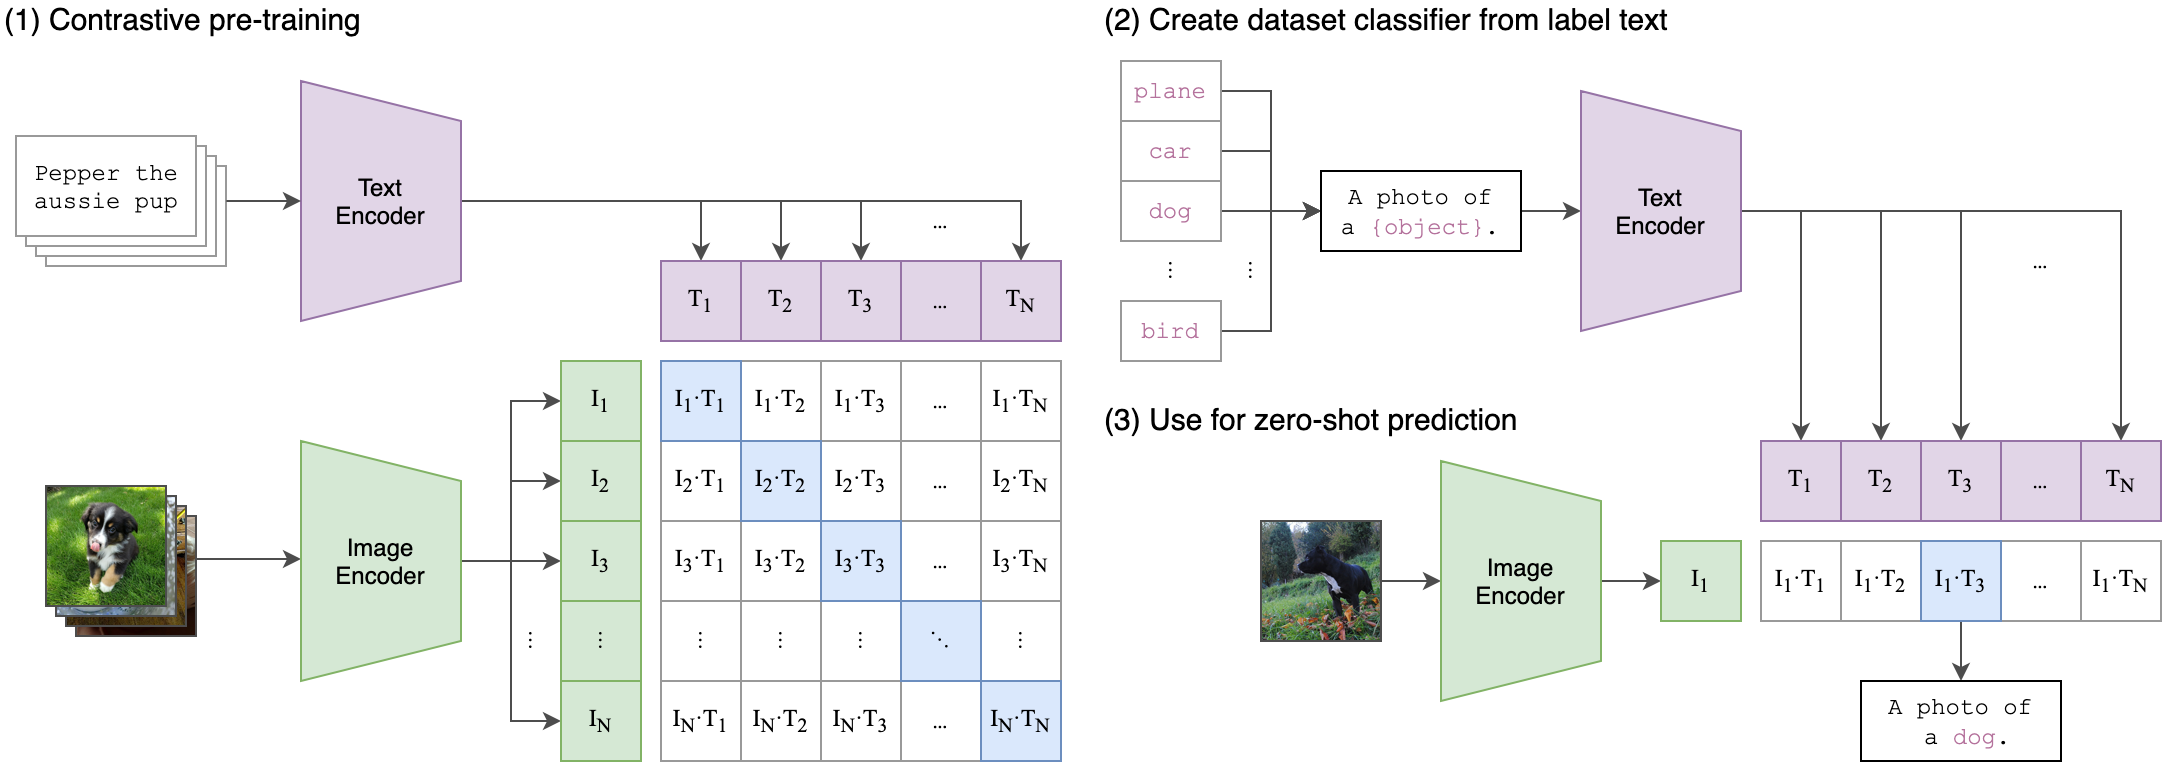
\includegraphics[width=0.8\textwidth]{imgs/CLIP.png}
	\caption{CLIP workflow}
	\label{fig:clip_architecture}
\end{figure}

The reason why these models work so well is because of the millions of image-text pair instances used for training and due to the model's ability to learn and deal with statistical spatial correlations that are shown both in the images and texts.

The dataset the model was trained on is a \textit{WebImageText} (WIT) containing more than 400 million pair instances scraped from the internet, almost half a million text queries and more than 20,000 image-text pairs as query. All of those queries were generated by the most frequent words of the english Wikipedia and then extended using bigrams. The dataset remains private and has never been released. 

Last but not least, images are preprocessed by dividing them into the RGB (reed, green and blue) channels and normalizing the values so they fall between range 0 to 1. Finally those values are merged with the mean and standard deviation of the images from the training dataset. In case the input image does not have the desired resolution (224x224 usually) the image is scaled by \textit{bicubic interpolation} \cite{wiki:bicubic_interpolation} to the shorter sides is the same as the native resolution, and then the central square of the image is cropped out.

%%%%%%%%%%%%%%%%%%%%%%%%%%%%%%%%%%%%%%%%%%%%%%%%%%%%%%%%%%%%%%%%%%%%%%%%%%%%%%%%%%%%% 

\section{Modality Bridging and Pseudo-Tokens}
\subsection{Modality bridging mechanism}
The bridge briefly mentioned in previous sections, serves as the "mathematical handshake" between the visual and linguistic domains. Because the vision encoder and the LLM are often trained independently, their output dimensions and feature spaces rarely match. It's in those scenarios where the \textit{dimensionality alignment} technique is applied. For example, an encoder such as ViT-L/14 may produce embeddings in a 1024-dimensional space (1024 embedding size), whereas a Llama-based LLM requires 4096-dimensional inputs.

To deal with different size embeddings, several algorithms have been developed, being the \textit{Manifold alignment} \cite{wiki:manifold_alignment} one of them. This algorithm assumes that both the image and textual data sets exist in different high-dimensional spaces, still they share an underlying common semantic structure, also called \textit{manifold}. The bridge's true purpose is to find a mapping that preserves the local geometric relationships of the two disparate sets. By minimizing the distance between related points while preserving the intrinsic structure of each domain. A great result would indicate the ability of the model to surpass the modality gap and project the same token close to each other across all modality spaces. 

\subsection{Pseudo-Tokens}
Once the different embeddings are aligned, tokens are referred as \textit{pseudo-tokens} or \textit{visual tokens}. There is an interesting paper where this kind of tokens are analyzed more in depth, I am talking about the \textit{A Sentence is Worth 128 Pseudo Tokens: A Semantic-Aware Contrastive Learning Framework for Sentence Embeddings
} paper \cite{tan2022sentenceworth128pseudo}. The study argues that a single sentence embedding is still not enough to capture visual complex meaning, it states that is necessary to use a fixed number of these new generated pseudo-tokens to actually represent a concept or image. In the context of VLMs, pseudo-tokens ensure that the LLM is able to look for different parts of the visual manifold as if they were a structure sequence of words, making easier to align between high-dimensional visual and semantic features. 

When it comes to practical cases, this alignment is implemented through varying levels of architectural complexity. The simplest and most common approach, seen in models like LLaVA, utilizes a \textit{linear projection} or a shallow \textit{multi-layer perceptron} (MLP) to perform the manifold mapping. On the other hand, more advanced architectures like Flamingo or BLIP-2 use bottleneck structures such as the \textit{perceiver resampler} or the \textit{q-former}. These use a set of learned queries to attend to the encoder's output, effectively summarizing the visual space into a fixed, manageable number of pseudo-tokens. This prevents the LLM from being overwhelmed by the high-resolution raw output of the vision encoder, especially when dealing with high-resolution images or video sequences.

%%%%%%%%%%%%%%%%%%%%%%%%%%%%%%%%%%%%%%%%%%%%%%%%%%%%%%%%%%%%%%%%%%%%%%%%%%%%%%%%%%%%%

\section{Training Strategies in VLMs}
Vision language models are trained not only in a single step process, but in a multi-stage training workflow, starting from the alignment of two disparate data modalities going to refining the model's ability to deal with natural instructions. The methodologies can be categorized into paradigms:

\subsection{Contrastive Pre-Training}:
The core of contrastive methods is the idea  of learning how to contrast between pairs of similar and dissimilar data points \cite{rethmeier2021primercontrastivepretraininglanguage}. A pair of similar data points is called positive sample if both points are different representations of the same data instance, in our case multimodal representations of the same instance. Whereas the negative samples are those pairs in which the data points belong to different examples. While computer vision methods learn from input-input (image-image) pairs and natural language processing methods deal with input-output (text, label) pairs, vision language models receive input-input (text, image) pairs. Previously mentioned models such as \textit{CLIP} \cite{radford2021learningtransferablevisualmodels}, apply this learning approach to maximize the \textit{cosine similarity} distance metric between matching image-text pairs in a shared embedding space, aiming to maximize the metric for the positive samples while minimizing the negative ones. The loss function used is the \textit{cross-entropy} function.

\subsection{Generative Pre-Training}
While contrastive learning focuses on aligning data points from different modalities in a shared single embedding space, generative pre-training shapes that task as a sequence-to-sequence problem. Using thie \textit{Prefix Language Modeling} (PrefixLM) approach \cite{wang2022simvlmsimplevisuallanguage}, the model receives a prefix consisting of a pair of image patches and a text sequence. The goal of the model is to predict the continuation of that textual sequence, just like \textit{seq2seq} models like \textit{RNNs} and \textit{LSTMs} try to predict. The loss function used is the negative log-likelihood loss, identical to the ones used in large language models like \textit{GPT}:
% loss function formula
$$\mathcal{L}_{PrefixLM} = -\sum_{t=1}^{|y|} \log P(y_t \mid y_{<t}, x_{prefix})$$
where $x_{prefix}$ represents the combined image and text prefix and $y_{t}$ is the text token at time $t$.

\subsection{Visual Instruction Tuning}
This strategy involves fine tuning the model with smaller datasets of higher quality, usually being (instruction-following) pairs where humans ask questions and the model replies. Supervised fine-tuning and parameter-efficient fine tuning methods are the most used ones, where only a small subset of the parameters is updated to avoid the LLM to forget its original knowledge. 

\subsection{Vision Language Models Training Paradigm}
When it comes to the training process of VLMs there are two main strategies to be adopted, strategies which will be discussed and which are visible in the referenced image below \ref{fig:scratch_vs_llm_backbone}. Those paradigms are no other than training a vision language from scratch versus starting from the base point of a pre-trained large language model as a frozen backbone. In the following section the procedures, differences and when to use each case will be studied.

\subsubsection{Training a VLM from Scratch}
Training the whole vision vision language model from zero differs significantly from starting from the base of having a pre-trained LLM. Usually a different training procedure and methodologies are applied, methodologies as the ones mentioned still \textit{contrastive pre-training} is the most used approach combined with \textit{self-supervised learning} techniques \cite{li2025surveystateartlarge}. The training procedure would be the ordinary one, showed in the upper side of schema on the referenced image. Consisting on training both encoders, getting the respective vectors and applying contrastive alignment to form the final shared vector space. 

\subsubsection{Starting from a pre-trained LLM}
On the other hand, starting from the checkpoint of already having a pre-trained large language model reduces or at least modifies the conventional training workflow. The text embeddings taken from the text encoding would be directly fed into the LLM without any previous alignment, however, there are two different alternatives to tackle the alignment task in for this training workflow variant: 

\begin{enumerate}
	\item \textbf{The Projector}: maps visual features extracted from the vision encoder with the text embeddings returned from the large language model, mapping which usually consists of multilayer perceptron (MLP) layers responsible for transforming high-dimensional visual representations into compact embedding tokens to be aligned with textual modality. The projector can be trained alongside the rest of the model or freezing the LLM in order to preserve the pre-trained knowledge. Among the modern models which follow this paradigm we have \textit{LLaVa, Qwen-VL} and \textit{Nvidia VLM}. 
	
	\item \textbf{Optimization Strategies (Joint vs Freeze Training)}: the second task involves updating a portion of the weights while freezing the others. \textit{Joint training} refers to updating the weights of all components of the model in parallel without freezing any (including the weights of the LLM and projector layers), approach taken by models such as \textit{Flamingo}. \textit{Freeze training} on the other hand, selectively freezes some components of the model during training, with the aim of preserving knowledge obtained prior to the training to be adapted to new tasks. The most common strategies are freezing the pre-trained vision encoders while fine-tuning the projector layers, gradually "unfreezing" the frozen parameters. 
\end{enumerate}

% argazkia azaldu scratch vs llm_backbones
\begin{figure}[H]
	\centering
	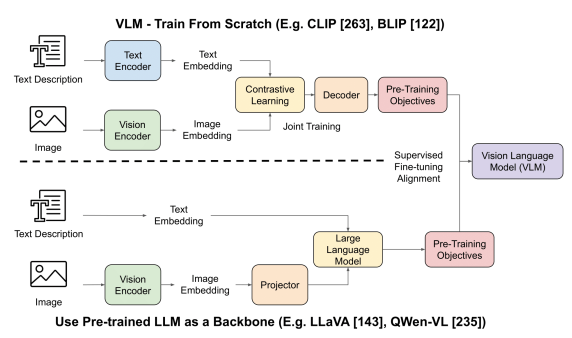
\includegraphics[width=.8\textwidth]{imgs/train_scratch_vs_llm_backbone.png}
	\caption{VLM trained from scratch vs training strategy using a pre-trained LLM as backbone}
	\label{fig:scratch_vs_llm_backbone}
\end{figure}

%%%%%%%%%%%%%%%%%%%%%%%%%%%%%%%%%%%%%%%%%%%%%%%%%%%%%%%%%%%%%%%%%%%%%%%%%%%%%%%%%%%%%

\section{Current SOTA VLMs}
The current vision language models are not judged exclusively by their ability to align image-text pairs, but by their system level efficiency, long context reasoning and architecture. This section will analyze the leading \textit{SOTA} models of the last years, models which represent the various approaches to the modality gap. Furthermore, these models have started to be implemented in chatbots to support multimodality user interaction. 

\subsection{State of the Art Models}

Following the same structure redacted in paper \textit{A Survey of State of the Art Large Vision Language Models: Alignment, Benchmark, Evaluations and Challenges} \cite{li2025surveystateartlarge}, some of the key models will be listed in a table form, alongside the metrics used to compare the models used in the paper.  

% table for vlm sota models comparison
\begin{table}[H]
	\centering
	\small
	\begin{tabular}{|>{\centering\arraybackslash}p{2.1cm}|c|>{\centering\arraybackslash}p{2.1cm}|>{\centering\arraybackslash}p{2.1cm}|c|>{\centering\arraybackslash}p{2.4cm}|>{\centering\arraybackslash}p{1.9cm}|}
		\hline
		\textbf{Model} & \textbf{Year} & \textbf{Architecture} & \textbf{Training Data} & \textbf{Params} & \textbf{Vision Encoder} & \textbf{Backbone} \\ \hline
		Flamingo & 2022 & Encoder-decoder & M3W, ALIGN & 80B & Custom & Chinchilla \\ \hline 
		BLIP/2 & 2022/23 & Encoder-decoder & COCO, Visual Genome & 223M-400M & ViT-B/L/g & Pretrained from scratch \\ \hline 
		LLaVA-1.5 & 2023 & Decoder-only & COCO & 13B & ViT-L/14 & Vicuna \\ \hline
		CogVLM & 2023 & Encoder-decoder & LAION-2B, COYO-700M & 18B & CLIP ViT-L/14 & Vicuna \\ \hline
		Gemini & 2023 & Decoder-only & Undisclosed & Undisclosed & Undisclosed & Undisclosed \\ \hline
		GPT-4V & 2023 & Decoder-only & Undisclosed & Undisclosed & Undisclosed & Undisclosed \\ \hline
		Qwen2-VL & 2024 & Decoder-only & Undisclosed & 7B-14B & EVA-CLIP ViT-L & Qwen-2 \\ \hline
	\end{tabular}
	\caption{Architectural comparison of representative SOTA Vision-Language Models extracted from referenced paper, including some of the key models.}
	\label{tab:vlm_comparison_main}
\end{table}

These are the models I have wanted to highlight, let's dive a little bit deeper into their interesting features:

\begin{enumerate}
	\item \textbf{Flamingo}: represents a foundational step in the transition towards generative VLMs built on top of frozen LLMs. Its key contribution was the \textit{Perceiver} architecture covered in section \ref{sec:perceiver}. This design, as mentioned, allows the pre-training knowledge to remain intact while the model learns visual context properties. 
	
	\item \textbf{BLIP-2}: introduced the \textit{querying transformer} (Q-Former) as a bridging module between a frozen image encoder and a frozen LLM. The Q-Former designs often purposely structure tokens, manipulate query sparsity or introduce language or structure-guided query selection \cite{li2023blip2}. This training strategy involving first aligning vision and language representations and then connecting the Q-Former output to the LLM makes BLIP-2 one if not the most parameter-efficient models, as the majority of weights keeps frozen during training.
	
	\item \textbf{LLaVa-1.5}: building upon the success of LLaVA, authors introduced the 1.5 version which incorporated several architectural and scaling techniques that enhance the performance. Compared to its predecessor, incorporated a broader and more diverse dataset and introduced more than 158k multimodal instruction-following pair examples for fine-tuning. Furthermore, it scaled images up to 336x336 pixel resolutions, enabling it to handle detailed visual content and capture finer aspects of images \cite{llava_medium_2023}. It stands as a baseline for open-source VLMs by utilizing a simple linear projection layer as the bridging layer. 
	
	\item \textbf{CogVLM}: introduced the \textit{Visual experts} architecture, able to reason complex spacial scenarios. Specially for robotic environments, it handles task of identifying relative position superb due to the layers in its transformers architecture destined for image processing. 
	
	\item \textbf{Gemini}: developed by Google, this model's defining feature is its massive context window, reaching up to 2 million tokens. This long-context capability enables the model to perform sophisticated temporal reasoning, identifying long-term patterns in agent behavior that models with smaller memory buffers would overlook. However, it's close source policy restricts the insight to its deep infrastructure. 
	
	\item \textbf{GPT-4V}: its strength lies in its world-grounding and common-sense reasoning, capable of interpreting high-level human instructions and translating them into logical sub-tasks. While its architecture remains undisclosed as the model mentioned beforehand, it serves as the primary benchmark for zero-shot performance in robotic task planning and complex scene description.
	
	\item \textbf{Qwen2-VL}: latest version of the Qwen family, stands as one if not the most powerful open-source vision language models out there. Apart from supporting multilingualism, stands out understanding long duration videos and images of different resolutions, it has been the model I have been experimenting with in the practical area of the work, due to its versatility and lightweight sub variants which preserve the overall performance.
\end{enumerate}

Looking at the models collected at table \ref{tab:vlm_comparison_main}, there are some properties that show the evolution and shift from some tendencies to others. Among those trends, there are some that could be highlighted:

\begin{itemize}
	\item \textbf{Connection paradigm shift}: there is a clear transition from alignment using \textit{multi-layer perceptrons} (MLPs) to a deeper integration. In earlier models like \textit{LLaVA-1.5}, the input images were treated as a set of tokens, whereas models like \textit{CogVLM} introduce approaches such as the 	\textit{Visual Experts} architecture. This architecture involves specialized visual encoders such as CLIP that provide distinct perception capabilities, enhancing the model's overall multimodal understanding. 
	
	\item \textbf{Closed and open source gap}: proprietary code models like \textit{GPT-4V} and \textit{Gemini} lead the multimodal reasoning leader boards, however, their black box nature limits their reproducibility and fine-tuning. Even if we know they follow a decoder-only architecture, there is no available information of the training data, number of parameters and their infrastructure. On the other hand, open source models offer a valuable insight of their properties such as the training data and number of parameters with total transparency. 
	
	\item \textbf{Efficiency and scalability}: the most recent tendencies lead to \textit{Mixture of Experts} (MoE) architectures. This technique allows to activate a portion of the total parameters during inference, achieving SOTA reasoning benchmarks while minimizing the computational cost. 
\end{itemize}

\subsection{Benchmarks}
The amount of VLM benchmarks has grown rapidly since 2022, moving from basic visual question answering to include a wider range of tests that better evaluate the model's multimodal capacities from more aspects.

% benchmark category-description table
\begin{table}[H]
	\centering
	\small
	\begin{tabular}{|>{\centering\arraybackslash}p{4.5cm}|>{\centering\arraybackslash}p{8.5cm}|}
		\hline
		\textbf{Category} & \textbf{Description} \\ \hline
		Visual text understanding & Model's ability o extract and understand texts within visual components. \\ \hline
		Visual math reasoning & Tests the model's skills to sole math problems in image forms \\ \hline
		Text-to-Image generation & Evaluates the image generation ability of the model \\ \hline 
		Hallucination & Evaluates the likelihood of models hallucinating on certain visual and textual inputs \\ \hline 
		Video understanding & Evaluates the VLM's ability to understand videos or sequence of images. \\ \hline 
		Visual reasoning, understanding, recognition and question answering & Evaluates the model's ability to recognize objects, answer questions and reason through both visual ant textual information \\ \hline
	\end{tabular}
	\caption{Categorization of standard benchmarks used to evaluate SOTA VLMs.}
	\label{tab:benchmarks}
\end{table}

Those are some of the 95 benchmarks covered in 13 categories for VLM evaluation collected in the mentioned study. Nevertheless, most of those VLM testing categories are still pretty far from the practical evaluation in the real world applications, such as scene understanding and autonomous driving. 

\subsubsection{Benchmark Data Collection} 
Those benchmarks are collected from a ton of datasets, the datasets used for vision language model benchmark evaluations are typically created using one of three data collection pipelines:

\begin{enumerate}
	\item \textbf{Fully human-annotated datasets}: are created thanks to having humans collecting or generating adversarial test questions sourced from diverse subjects and fields. For some studies such as \textit{Massive Multi-discipline Multimodal Understanding} (MMMU) \cite{yue2024mmmumassivemultidisciplinemultimodal}, more than 50 college students belonging to different disciplines were gathered to extract questions from textbooks and reading material. The issue with this method of data extraction is the scalability and time consume problem. 
	
	\item \textbf{Partially human-annotated datasets scaled up with synthetic data generation and partially validated by humans}: Synthetic data usage has become handy to quickly scale up the dataset sizes. Workflows often consist on using human written examples to be fed to a LLM to generate more adversarial question and answer examples. In the case of VLMs, image and video data are
	often paired with captions, which are used by authors as context to prompt LLMs to extract answers and generate questions. However, LLMs are not always accurate and may produce unfaithful content or hallucinations without human supervision. To tackle this low-fidelity issues automatic filtering pipelines were developed and crowd worker validation was used. 
	
	\item \textbf{Interaction in the Simulator}: mainly targeted at VLM benchmarks in robotics, it gathers data for training and evaluation by assessing the VLM-powered agents online. Such a data generation method is applicable for the scenarios in which human-labeled datasets or synthetic ones are not feasible to acquire, and the data follows some common rules like physical laws. The outputs tend to the most robust, nevertheless, the potential \textit{sim2real} gap might exist when transplanting the terminal VLM into real world-applications. 
\end{enumerate}

\subsubsection{Evaluation Metrics}
After collecting the data for benchmark evaluation, it's benchmark evaluation time. VLM benchmark evaluation metrics tend to be automatic to support repeated use at scale, and often influence the question formats used in the benchmark. The following are the most relevant metrics used for vision language benchmark evaluation. 

\begin{itemize}
	\item \textbf{Answer matching}: widely used for both open and close-ended question types. In order to evaluate the "perfect match" in practice, articles and unnecessary spaces are removed from both sentences and check if the normalized predicted answer is contained in the normalized "gold answer". Natural language evaluation metrics such as \textit{ROUGE, $F_{1}$} and \textit{BLEU} started being used, still their performance decayed when the generative LLMs started producing larger and more complex correct answers.
	
	\item \textbf{Multiple choice}: this metric involves selecting an answer from a set of possible correct options, options where often distractive answers are injected to confuse the model and enhance its reasoning capability towards these little tricks. Nevertheless, the evolution of the large language models have led to not necessarily needing to have the set of possible options in order to get the correct answer. 
	
	\item \textbf{Image/Text similarity score}: score to evaluate the alignment across the generated image and their corresponding textual description, commonly used in the image generation benchmark. Using \textit{CLIPScore} \cite{hessel2022clipscorereferencefreeevaluationmetric} for image-text alignment evaluation or \textit{ROUGE} for caption matching. I want to stop on CLIPScore, being a cross-modal retrieval model trained on (image-text) pairs for evaluation purposes, the evaluation formula it uses is the following one: 
	$$CLIP-S(\mathbf{c}, \mathbf{v}) = w \cdot \max(\cos(\mathbf{v}, \mathbf{c}), 0)$$
	where $\mathbf{c}$ and $\mathbf{v}$ are the text and image embeddings straight out from their respective encoders. Then the cosine similarity is applied to measure the distance between the two vectors and passed through an activation function to discard the negative similarity pairs and substitute them by value 0. Lastly, $w$ is a scaling factor.
	
	There is even a more advanced formula if dealing with references named \textit{RefCLIPScore}. After passing the embedding of each reference through CLIP, the result is a set of reference embeddings $R$. Then, the score is computed by taking the \textit{harmonic mean} of \textit{CLIPScore} and taking the maximal reference cosine-similarity.
	
	$$RefCLIP\text{-}S(\mathbf{c}, \mathbf{R}, \mathbf{v}) = \text{H-Mean}\left(CLIP\text{-}S(\mathbf{c}, \mathbf{v}), \max_{r \in R} (\max(\cos(c\mathbf{c}, \mathbf{r}), 0))\right)$$
	
	Being the harmonic mean formula a kind of average used for ratios and rates: 
	$$H\text{-}Mean(x_1, x_2, \dots, x_n) = \frac{n}{\sum_{i=1}^{n} \frac{1}{x_i}} = n \left( \sum_{i=1}^{n} x_i^{-1} \right)^{-1}$$
\end{itemize}

% figure of benchmark metrics
\begin{figure}[H]
	\centering
	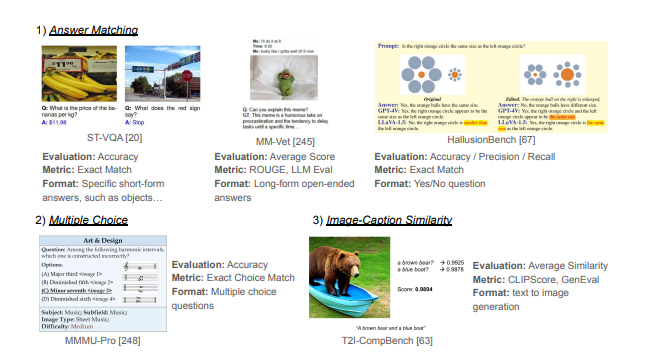
\includegraphics[width=1\textwidth]{imgs/benchmark_metrics.png}
	\caption{Most common benchmark evaluation metrics illustrated visually; showing \textit{answer matching, multiple choice} and \textit{image-caption similarity} graphical examples.}
	\label{fig:benchmark_metrics}
\end{figure}

\subsection{Vision Language Action (VLA) Models}
As the latest step of VLM evolutions, a new sub variant arose with the name of vision-language-action (VLA) models. Multimodal foundational models which include all the prior work of the VLMs, adding the actions space to the vision and language ones. With these models, given an input image or video of the robot's surroundings alongside a text instruction, the VLA directly outputs low-level robot action instructions to be executed to accomplish the task \cite{wiki_vla_2026}. 

The architecture of the VLA would stand as the standard VLM architecture just changing the decoder to an \textit{action decoder} which translates the latent VLM representation into continuous output actions to be directly applied on the robot. 

\begin{figure}[H]
	\centering
	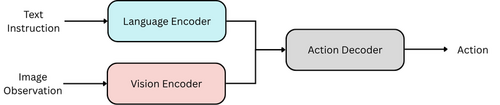
\includegraphics[width=.6\textwidth]{imgs/VLA.png}
	\caption{Standard vision language action model architecture.}
	\label{fig:vla_architecture}
\end{figure}

\subsubsection{OpenVLA}
Among the most popular vision language action models, there is model \textit{OpenVLA}, a 7B parameter VLA model trained on almost a million robot demonstration instances \cite{kim2024openvlaopensourcevisionlanguageactionmodel}.

When it comes to the training of the model, a pre-trained VLM was used as a backbone and fine-tuned for robot action prediction. The input replicates the same (image-text) pair procedure seen in VLMs but the output now consists of a string containing the robot action to take. In order to get prediction by the VLM backbone, the robot actions are represented in the output space of the LLM by mapping continuous actions to discrete tokens used by the language model's tokenizer. 

\begin{figure}[H]
	\centering
	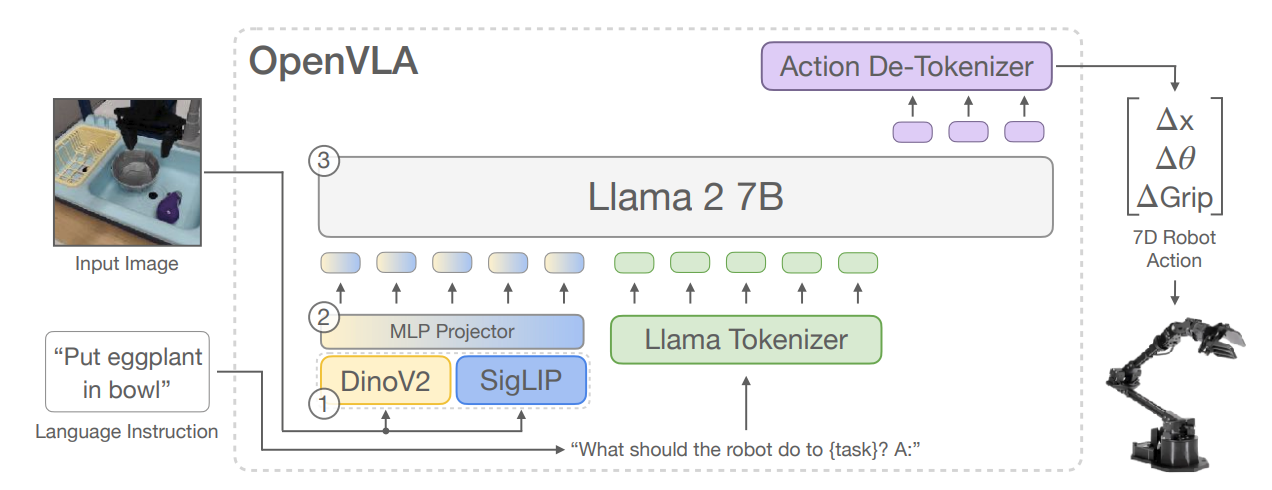
\includegraphics[width=.8\textwidth]{imgs/OpenVLA_architecture.png}
	\caption{Given an image observation and a language instruction, the model
		predicts 7-dimensional robot control actions. The architecture consists of three key components: a vision encoder, a projector that maps visual features to
		the language embedding space, and the LLM backbone, in this case, a Llama 2 7B-parameter large language model.}
	\label{fig:open_vla_architecture}
\end{figure}

However, current VLA models still face significant challenges regarding high-frequency control and multi-agent coordination. Most VLAs are trained for single-arm manipulation and struggle with the low-latency requirements of complex dynamic environments. In the context of this project, while these new vision language action architectures represent the SOTA in embodied AI, the integration of a vision language models into multi-agent robotic systems represent a more robust combination, reason why I decided to stick to VLMs for the part of complex reasoning due to their stability over these newer models. 

%%%%%%%%%%%%%%%%%%%%%%%%%%%%%%%%%%%%%%%%%%%%%%%%%%%%%%%%%%%%%%%%%%%%%%%%%%%%%%%%%%%%%

\section{Reinforcement Learning and Multi-Agent Systems in Robotics}
In the context of machine learning, RL is concerned with how an intelligent agent should take actions in a dynamic environment in order to maximize a reward signal. The agent must make decisions between trying new actions to learn more about the environment or using current knowledge of the environment to take the best action, balancing the exploration/exploitation trade.  

\begin{figure}[H]
	\centering
	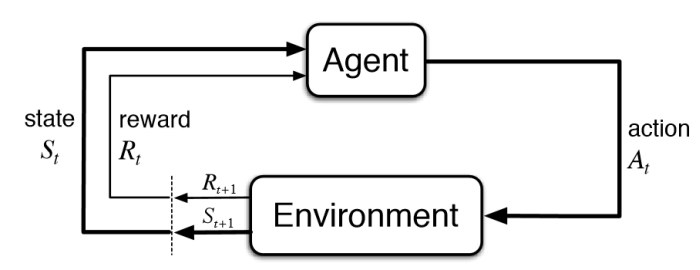
\includegraphics[width=0.5\textwidth]{imgs/reinforcement-learning-fig1-700.jpg}
	\caption{Basic RL worfklow schema: the agent iteratively maps states to actions by maximizing a cumulative reward signal through trial and error interaction.}
	\label{fig:rl_schema}
\end{figure}

Particularly their combination with deep neural networks, referred to as \textit{deep reinforcement learning} (DRL) have shown remarkable capabilities in solving the most complex decision-making problems even with the high-dimensional observations in domains such as board games, video games, healthcare and recommendation systems \cite{tang2024deepreinforcementlearningrobotics}.  

\subsection{Reinforcement Learning in robotic environments}
Reinforcement learning offers to robotics a framework and set of tools for the design of sophisticated and hard-to-engineer behaviors. The successes of combining deep neural networks for reinforcement learning policy training underscore the potential of DRL for controlling robotic systems with
high-dimensional state or observation space and highly nonlinear dynamics to perform challenging tasks that conventional decision-making, planning, and control approaches (e.g.,
classical control, optimal control, sampling-based planning) cannot handle effectively. Furthermore, robots need
to complete tasks in the physical world, which presents additional challenges. It is often
inefficient and/or unsafe for the RL agents to collect trial-and-error samples directly in the
physical world, and it is usually impossible to create an exact replica of the complex real
world in simulation.

\subsection{RL and VLM Combination}
Reinforcement learning in complex scenarios is time consuming and as massive interaction steps are needed to learn optimal policies, and even if VLA seem promising to reduce time complexity, they still are immature and don't perform well on low-level control scenarios \cite{wu2025teachingrlagentsact}. That is the reason why vision language models remain on the edge of helping models for reinforcement learning. Combining the reinforcement learning machine learning subfield with the architecture reviewed throughout the document, there has been an increasing trend towards combining both in order to form a more compact learning system. However, VLMs do not tend to control the agent's engine directly, rather they serve as an "orchestrator" which transfer their reasoning knowledge obtained from the environment to the agent. Vision language models can be applied into reinforcement learning as several approaches.

\subsubsection{Vision Language Models as Action Advisors}
In many studies vision languages models are proposed as action advisors for online reinforcement learning, leveraging the knowledge of VLMs to provide action suggestions for RL agents. Unlike previous methods, actions are proposed rather than designing heuristic rewards. 

As illustrated in the comparison image below \ref{fig:VARL_comparison} for a robotic-arm grasp policy, zero-shot vision-language-action models tend to produce biased still inaccurate actions which partially approach task success. When it comes to the policy obtained in the early stages of a RL, often reflect near-random behaviors. In contrast to the previous two approaches, VLM as action advisor for online reinforcement learning (VARL) achieves the most accurate grasping with just a few interactions and converges efficiently. 

\begin{figure}[H]
	\centering
	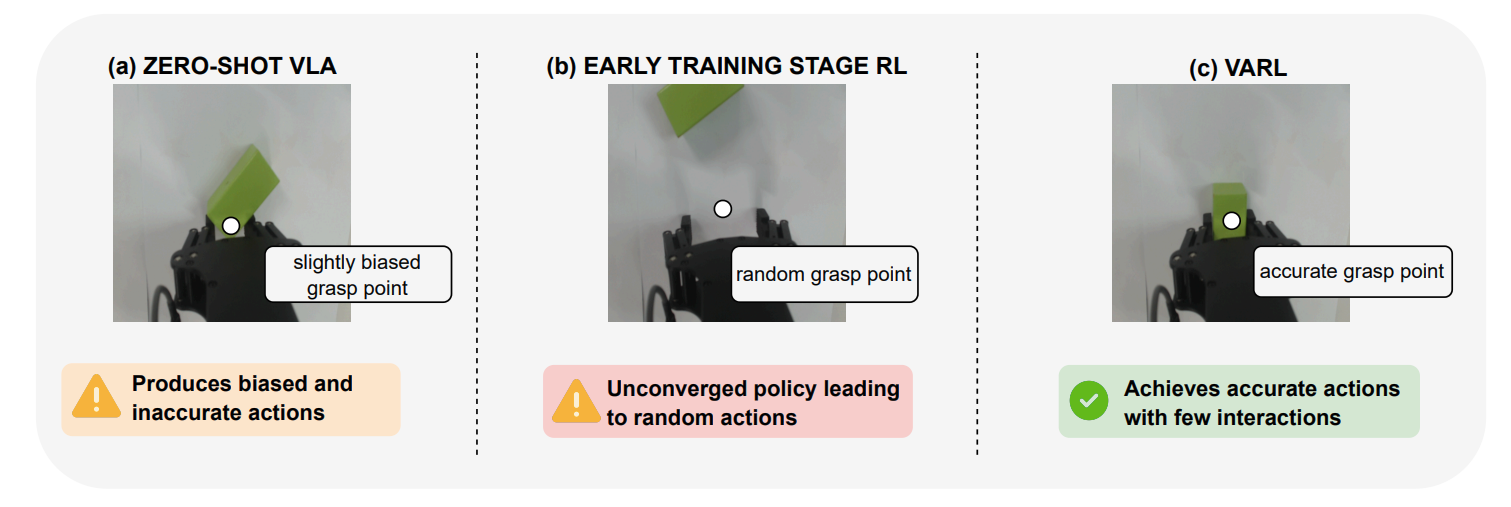
\includegraphics[width=.8\textwidth]{imgs/VARL.png}
	 \label{fig:VARL_comparison}
	 \caption{Different RL training approach comparison}
\end{figure}

\subsubsection{VLM-based Reward Shaping}
Another promising approach is to employ VLMs and LLMs as reward designers. Rather than suggesting direct actions, these models are used to shape or generate reward signals that guide reinforcement learning agents. Typically those rewards are generated by letting large language models read the task descriptions. \textit{Eureka} and \textit{Text2Reward} are some of the models which take that approach. 

\subsection{Multi Agent Robotic Systems (MARS)}
Multi-agent robotic systems (MARS) are distributed autonomous systems where multiple robotic agents cooperate, compete, or interact to solve complex tasks that are too large, dynamic, or unpredictable for a single robot.  Unlike centralized AI, MARS distributes intelligence across the whole network, allowing each agent to make decisions based on local information, which enhances scalability, adaptability, and fault tolerance.

Where the core challenge of MARS actually lies is in the coordination among agents, to address this modern multi-agent frameworks often go for one of two algorithm approaches: centralized and decentralized learning \cite{yu2022surprisingeffectivenessppocooperative}. Centralized methods directly learn a single policy to produce the joint actions of all agents, whereas in decentralized learning each agent optimizes its rewards independently. \textit{Centralized training and decentralized execution} (CTDE) algorithms fall in between these two approaches. This approach enables the agent to learn global information during the training phase in simulation while maintaining autonomy during execution. By using a centralized critic that observes the global state and the actions taken by the agents during training, the learning process becomes more stable. Nevertheless, the actors being the robots only have access to their local actions, enabling them to not rely on the critic once deployed on inference. 

\subsubsection{Multi Agent Reinforcement Learning (MARL)}
MARL addresses the sequential decision-making problem of multiple autonomous agents which operate in a common shared environment, each of which aims to optimize its own long-term reward by interacting with the environment and the other agents \cite{zhang2021multiagentreinforcementlearningselective}. There are two different but closely related theoretical frameworks for MARL:

\begin{enumerate}
	\item \textbf{Markov/Stochastic Games}: MDP generalization that captures the interconnection of multiple agents. In a Stochastic Game, the environment transitions between states based on the joint actions of all agents. Each agent receives a reward that depends not only on its own action and the current state but also on the actions of the others'. This model is particularly useful for representing continuous or long-term interactions in dynamic environments where the state is fully or partially observable at each discrete time step.
	
	\item \textbf{Extensive-Form Games}: This framework represents the interaction as a tree structure, capturing the sequential nature of decision-making. Unlike Stochastic Games, Extensive-Form Games are ideal for modeling scenarios where agents move in a specific order or where there is imperfect information. For instance when some agents do not know the previous moves of others. 
\end{enumerate}

Multi-agent RL suffers from several theoretical challenges in addition to those raised in single-agent reinforcement learning. Being those the non-unique learning goals of the agents in the environment, the non-stationarity of the environment caused by multiple agents learning concurrently, scalability issues and structural information issues.

\subsection{Sim to Real Frameworks}
Sim2Real frameworks are computational systems designed to transfer control policies and models trained in simulated environments to real world applications. Generally implementing reinforcement learning in virtual environments, these frameworks seek model transferability of the knowledge obtained by the agents into the real world, trying to break that \textit{reality gap} consisting of physical, visual and dynamic discrepancies between the simulator and the real world. Among the state of art frameworks, there are several advanced options to choose from. 

\begin{itemize}
	\item \textbf{Sim2Real-AD}: is a modular framework specially designed for autonomous driving that enables zero-shot deployment of vision language model guided reinforcement learning policies \cite{huang2026sim2realadmodularsimtorealframework}. The framework is known for implementing SOTA technology such as a \textit{geometric observation bridge} (GOB) for converting monocular camera images into the simulator's \textit{bird eye view} (BEV) representation and a \textit{physics-aware action mapping} (PAM) to translate policy outputs into physical commands.
	
%	\begin{figure}[H]
%		\centering
%		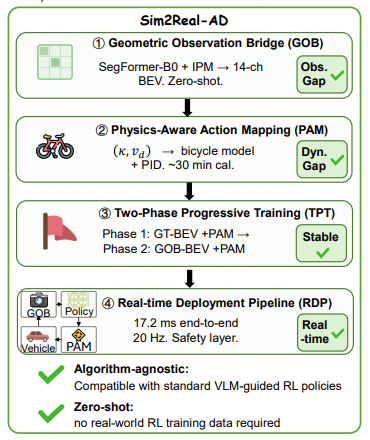
\includegraphics[height=.5\textwidth]{imgs/sim2realAD.png}
%		\label{fig:sim2realAD}
%		\caption{In order to tackle sim-to-real challenges}
%	\end{figure}
	
	\item \textbf{EAGERx}: provides a unified software pipeline for robot learning that supports multiple simulation engines and integrates state, action, and time-scale abstractions. The open source project available in GitHub \cite{eagerx2023}, enables the user to define environments as graph nodes visualized in a GUI. Policies are trained in simulation and zero-shot evaluated on real systems and EAGERx's design allows users to create complex environments using modular compositions. 
	
	\item \textbf{NVIDIA IsaacSim}: NVIDIA's physics simulation platform built on top of \textit{NVIDIA Omniverse}, which will in fact be the selected framework for the practical field of the project. IsaacSim enables zero-shot sim2real transfer offering accurate physics simulation for realistic robot dynamics, synthetic data generation with domain randomization to train more robust models and it also supports reinforcement and imitation learning. On top of that it is integrated with \textit{Isaac ROS} and \textit{Isaac Lab} for real time deployment. Furthermore, Isaac Sim leverages NVIDIA RTX technology for ray-traced rendering, providing the photorealistic visual inputs essential for the effective reasoning of VLMs. The platform is built on the \textit{Universal Scene Description} (USD) framework, which facilitates seamless asset interoperability and scene management. Crucially for multi-agent research, Isaac Sim enables massively parallel simulation by executing physics and perception pipelines entirely on the GPU, allowing for the simultaneous training of large robotic fleets in complex, shared environments. As a quick note, I have preferred to keep the overview of the framework simple in this section in order to deepen in the corresponding chapter due to its importance and links to the practical environment development. 
\end{itemize}

% Finally, a conclusion paragraph for the SOTA chapter
In conclusion, this chapter has reviewed the transition from static vision-language reasoning to the embodied robot action. While current vision-language-action models seem promising, the complexity of multi-agent cooperation in critical environments requires a modular approach. The following chapters will detail how the reasoning capabilities of the selected VLM are integrated in multi-agent environments within NVIDIA IsaacSim to achieve coordinated robotic tasks.